\documentclass[conference]{IEEEtran}
\IEEEoverridecommandlockouts

\usepackage{cite}
\usepackage{amsmath,amssymb,amsfonts}
\usepackage{algorithmic}
\usepackage{graphicx}
\usepackage{textcomp}
\usepackage{xcolor}
\usepackage{booktabs}
\usepackage{multirow}
\usepackage{url}
\usepackage{hyperref}

\hypersetup{
    colorlinks=true,
    linkcolor=blue,
    filecolor=magenta,      
    urlcolor=cyan,
    citecolor=blue,
}

\def\BibTeX{{\rm B\kern-.05em{\sc i\kern-.025em b}\kern-.08em
    T\kern-.1667em\lower.7ex\hbox{E}\kern-.125emX}}

\begin{document}

\title{FactLens: Atomic Claim-Level Hallucination and Grounding Verification for Large Language Model Outputs}

\author{\IEEEauthorblockN{Goutham Reddy}
\IEEEauthorblockA{\textit{Department of Computer Science and Engineering} \\
\textit{Indian Institute of Information Technology, Design and Manufacturing (IIITDM), Kurnool}\\
Andhra Pradesh, India \\
Email: goutham.reddy@iiitk.ac.in}
}

\maketitle

\begin{abstract}
Large Language Models (LLMs) frequently generate plausible-sounding yet factually unsupported or contradictory statements, commonly termed hallucinations. Existing automated evaluation paradigms predominantly rely on surface lexical overlap metrics (e.g., ROUGE, BLEU) or document-level Natural Language Inference (NLI) cross-encoders. However, feeding entire multi-sentence documents directly into standard transformer cross-encoders introduces severe \textit{attention dilution}: localized factual anomalies—such as numerical swaps, entity distortions, or subtle extrapolations—are overshadowed by dominant background agreement across the surrounding context. To overcome this limitation, we present \textbf{FactLens}, a modular, four-stage atomic claim-level grounding verification pipeline. FactLens decomposes AI-generated text into isolated, single-fact atomic claims, retrieves the top-$k$ most salient source premises using a dense sentence bi-encoder (\texttt{all-MiniLM-L6-v2}), verifies each claim–premise pair via a high-capacity cross-encoder (\texttt{DeBERTa-v3-base-mnli-fever-anli}), and computes a calibrated, non-linear Grounding Trust Score ($\text{GTS}$). Evaluated on a curated, multi-domain benchmark of 30 challenging cases spanning clinical abstracts, financial earnings, Indian policy briefings, and systems documentation, FactLens improves Macro F1-score from 59.3\% (baseline whole-document NLI) to \textbf{95.9\%} ($+36.6\%$ absolute gain) and accuracy from 60.0\% to \textbf{96.7\%} ($+36.7\%$). Crucially, on critical numerical distortions and extrapolated fabrications, FactLens achieves \textbf{100.0\%} F1 detection while maintaining sub-second batched inference ($380.1\text{ ms}$).
\end{abstract}

\begin{IEEEkeywords}
Natural Language Processing, Hallucination Detection, Fact Verification, Natural Language Inference, Large Language Models, Atomic Decomposition.
\end{IEEEkeywords}

\section{Introduction}
Large Language Models (LLMs) based on generative autoregressive architectures have demonstrated extraordinary generation capabilities across text summarization, clinical question answering, code synthesis, and analytical report generation \cite{brown2020language, touvron2023llama}. Despite their generative fluency, their propensity to fabricate fictitious assertions—a phenomenon widely characterized as \textit{hallucination}—remains the single most formidable bottleneck hindering their enterprise and high-stakes deployment in healthcare, legal, and financial intelligence \cite{ji2023survey}.

Historically, automated grounding verification has depended on surface-level n-gram overlap metrics, notably ROUGE \cite{lin2004rouge} and BLEU \cite{papineni2002bleu}. While computationally negligible, lexical overlap metrics completely disregard semantic entailment: an LLM response may achieve a near-perfect ROUGE-1 score while inverting an interest rate direction, altering a drug dosage by an order of magnitude, or attributing an outcome to a competitor firm. 

To introduce semantic awareness, recent works adopted document-level Natural Language Inference (NLI) cross-encoders \cite{williams2018broad, laurer2022less}. In this naive configuration, the entire reference source document is concatenated with the entire generated text $(P=\text{Document}, H=\text{Summary})$ and passed through a transformer model. However, our empirical findings reveal that document-level cross-encoders suffer from severe \textbf{attention dilution}:
\begin{enumerate}
    \item When a paragraph contains three factually accurate sentences alongside one critical numerical distortion (e.g., reporting a 27.2\% margin instead of 7.2\%), the self-attention mechanism spreads probability mass across the majority token matches, yielding an erroneous aggregate verdict of \textit{Entailment}.
    \item When an LLM extrapolates unmentioned facts, document-level NLI defaults to \textit{Neutral}, failing to localize the precise hallucinated statement.
    \item Document-level scoring offers zero interpretability, leaving users unable to inspect which specific claim failed or where supporting evidence resides in the source text.
\end{enumerate}

To resolve these shortcomings, we present \textbf{FactLens}, an open-source, production-ready framework for fine-grained atomic claim-level hallucination verification. FactLens decomposes complex generated narratives into discrete, verifiable factual atoms, performs dense bi-encoder semantic retrieval against the source document, executes cross-encoder inference on isolated claim-evidence pairs, and calculates a calibrated Grounding Trust Score ($\text{GTS}$).

\textbf{Contributions:}
\begin{itemize}
    \item \textbf{Modular 4-Stage Architecture}: We design and implement an end-to-end pipeline featuring dual-mode atomic decomposition (offline syntactic rule engine and few-shot LLM API), dense bi-encoder evidence retrieval, and DeBERTa-v3 cross-encoder verification.
    \item \textbf{Calibrated Grounding Trust Score ($\text{GTS}$)}: We formulate an asymmetric scoring metric incorporating semantic retrieval confidence weighting and an exponential contradiction penalty $\Omega(K)$ that strictly penalizes factual falsehoods over missing evidence.
    \item \textbf{Multi-Domain Benchmark & Ablation Study}: We construct a rigorous 30-case multi-domain benchmark covering medical, financial, macroeconomic, and technical systems domains across four failure modes: Fully Grounded, Numerical Distortion, Entity/Attribute Swap, and Extrapolated Fabrication. FactLens demonstrates a $+36.6\%$ Macro F1 gain over whole-document baselines.
    \item \textbf{Auditable Open-Source Suite}: We deliver an interactive, presentation-ready Streamlit dashboard with inline color-coded document scanning, stacked softmax probability distributions, and JSON/Markdown audit artifact generation.
\end{itemize}

\begin{figure*}[t]
\centering
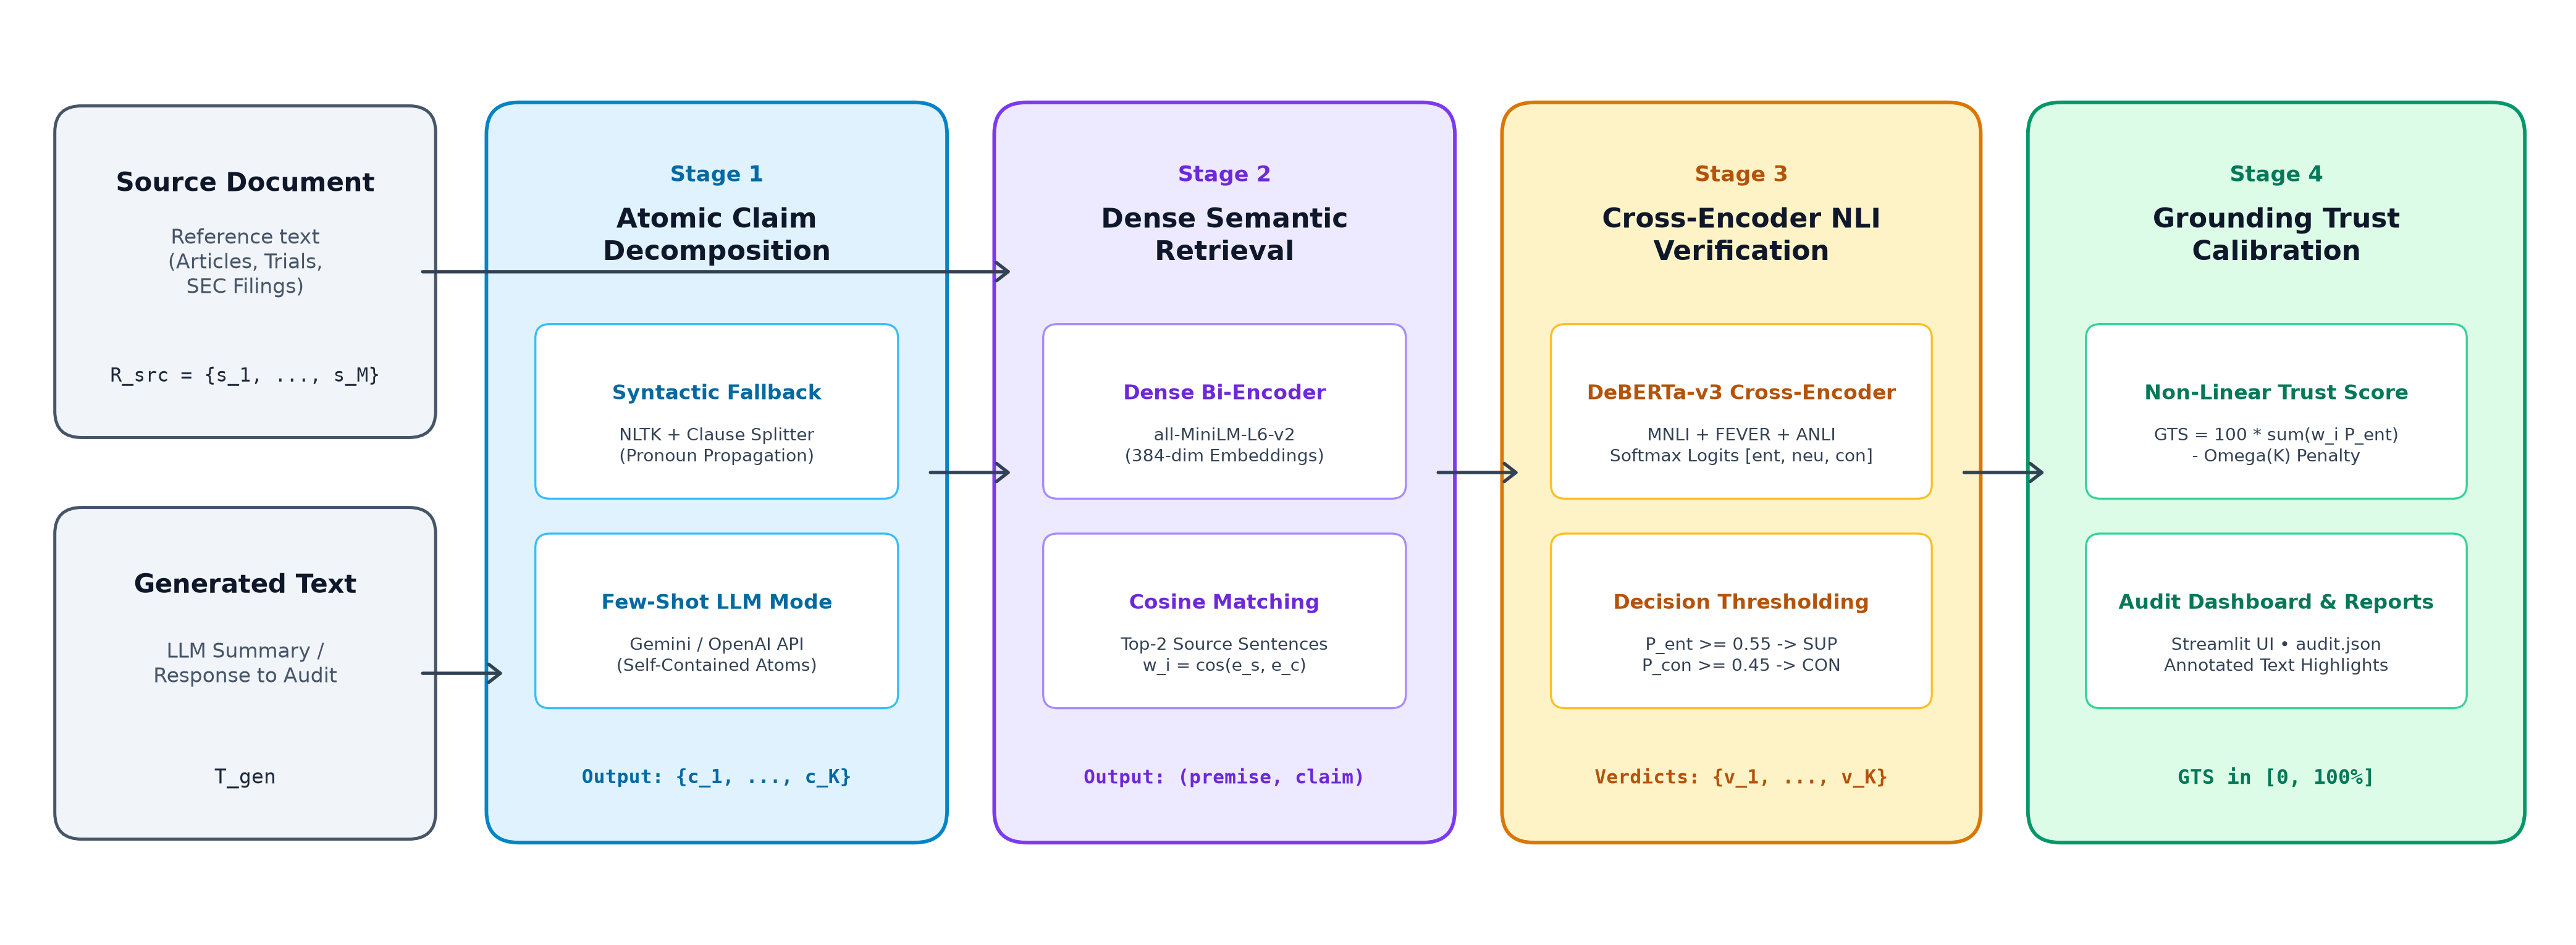
\includegraphics[width=0.98\linewidth]{figures/fig1_pipeline_architecture.png}
\caption{The FactLens 4-Stage End-to-End Verification Architecture: AI-generated text is parsed into discrete atomic claims, matched with salient source premises via dense MiniLM embeddings, verified through a DeBERTa-v3 cross-encoder, and calibrated into an overall Grounding Trust Score ($\text{GTS}$).}
\label{fig:architecture}
\end{figure*}

\section{Related Work}
\subsection{Hallucination Detection in Generative NLP}
Hallucination in natural language generation encompasses intrinsic hallucinations (contradicting the provided source context) and extrinsic hallucinations (asserting unverified information absent from the source) \cite{ji2023survey}. While sampling-based uncertainty estimation methods (such as SelfCheckGPT \cite{manakul2023selfcheckgpt}) assess consistency across repeated stochastic generations, they require multiple decoding passes, imposing prohibitive inference latency and API costs. Furthermore, black-box consistency checks cannot reference a definitive ground-truth source document.

\subsection{Fine-Grained Claim Decomposition}
Min et al. \cite{min2023factscore} pioneered FActScore for evaluating biography generation by prompting instruction-tuned models to break down paragraphs into atomic facts. While effective for open-domain factual recall against Wikipedia, FActScore relies heavily on expensive commercial LLM APIs for both decomposition and verification. FactLens distinguishes itself by implementing a hybrid dual-mode decomposition engine: a high-speed, rule-based syntactic engine utilizing clause boundary detection and pronoun resolution that operates entirely offline on consumer CPUs, accompanied by an optional few-shot LLM mode.

\subsection{Dense Retrieval and NLI Cross-Encoders}
Sentence-BERT \cite{reimers2019sentence} demonstrated that dual-encoder architectures with cosine similarity enable rapid, scalable semantic search over dense vector spaces. For premise-hypothesis verification, cross-encoders—such as DeBERTa-v3 \cite{he2021deberta} trained on multi-task NLI datasets (MNLI \cite{williams2018broad}, FEVER \cite{thorne2018fever}, and Adversarial NLI \cite{nie2020adversarial})—substantially outperform bi-encoders by modeling all-to-all cross-attention between token representations \cite{laurer2022less}. FactLens couples bi-encoder retrieval efficiency (\texttt{all-MiniLM-L6-v2}) with cross-encoder verification precision (\texttt{DeBERTa-v3-base-mnli-fever-anli}).

\section{System Methodology}
FactLens executes a sequential 4-stage pipeline that ingests a reference source document $R_{\text{src}}$ and an AI-generated text $T_{\text{gen}}$, producing an audit report of verified claims and an aggregate Grounding Trust Score ($\text{GTS}$). Fig.~\ref{fig:architecture} details the system architecture.

\subsection{Stage 1: Atomic Claim Decomposition}
Given a generated response $T_{\text{gen}}$, Stage 1 segments compound, multi-clause paragraphs into a set of $K$ self-contained, single-fact atomic claims:
\begin{equation}
T_{\text{gen}} \xrightarrow{\text{Decompose}} \mathcal{C} = \{c_1, c_2, \dots, c_K\}
\end{equation}

FactLens provides a dual-mode engine:
\begin{enumerate}
    \item \textbf{Syntactic Engine (Offline CPU Fallback)}: Performs sentence tokenization via NLTK, followed by rule-based clause splitting over coordinating conjunctions (\textit{and}, \textit{but}, \textit{whereas}) and relative pronouns (\textit{which}, \textit{who}, \textit{that}). When a clause lacks an explicit nominal subject, the syntactic engine performs backward pronoun propagation from the primary clause, ensuring each atom retains standalone semantic context.
    \item \textbf{LLM Engine (Few-Shot API)}: Utilizes structured few-shot prompting via Gemini or OpenAI APIs to resolve co-references and synthesize clean grammatical atomic assertions without hallucinating ancillary facts.
\end{enumerate}

\subsection{Stage 2: Dense Semantic Evidence Retrieval}
To verify claim $c_k \in \mathcal{C}$, the pipeline must locate the most pertinent factual evidence within the source document $R_{\text{src}}$. The source document is segmented into $M$ sentences $\mathcal{S} = \{s_1, s_2, \dots, s_M\}$.

Using the bi-encoder $\mathcal{E}_{\text{dense}}$ (\texttt{sentence-transformers/all-MiniLM-L6-v2}), we compute 384-dimensional dense semantic embeddings:
\begin{equation}
\mathbf{e}_{s_m} = \mathcal{E}_{\text{dense}}(s_m), \quad \mathbf{e}_{c_k} = \mathcal{E}_{\text{dense}}(c_k)
\end{equation}
The semantic similarity between source sentence $s_m$ and claim $c_k$ is evaluated via cosine similarity:
\begin{equation}
\text{sim}(s_m, c_k) = \frac{\mathbf{e}_{s_m} \cdot \mathbf{e}_{c_k}}{\|\mathbf{e}_{s_m}\|_2 \|\mathbf{e}_{c_k}\|_2}
\end{equation}

For each claim $c_k$, FactLens retrieves the top-$k$ candidate premises ($k=2$). If the maximum similarity falls below the semantic relevance threshold $\tau_{\text{sim}} = 0.25$, the claim is tagged as lacking relevant source grounding, circumventing unnecessary cross-encoder computation.

\subsection{Stage 3: Cross-Encoder NLI Verification}
For each retrieved premise-claim pair $(premise=s^*_k, hypothesis=c_k)$, FactLens invokes the cross-encoder $\mathcal{M}_{\text{NLI}}$ (\texttt{MoritzLaurer/DeBERTa-v3-base-mnli-fever-anli}). Tokens are concatenated with separation delimiters:
\begin{equation}
\mathbf{x} = \text{[CLS]} \circ s^*_k \circ \text{[SEP]} \circ c_k \circ \text{[SEP]}
\end{equation}
The model computes logits $\mathbf{z} \in \mathbb{R}^3$, transformed via Softmax into probabilities:
\begin{equation}
[P_{\text{ent}}, P_{\text{neu}}, P_{\text{con}}] = \text{Softmax}(\mathbf{z})
\end{equation}
FactLens assigns discrete labels according to calibrated decision boundaries:
\begin{equation}
\mathcal{V}(c_k) = 
\begin{cases} 
\text{SUPPORTED}, & \text{if } P_{\text{ent}} \ge \tau_{\text{ent}} \land P_{\text{ent}} > P_{\text{con}} \\
\text{CONTRADICTED}, & \text{if } P_{\text{con}} \ge \tau_{\text{con}} \land P_{\text{con}} > P_{\text{ent}} \\
\text{UNVERIFIED}, & \text{otherwise}
\end{cases}
\end{equation}
where empirical grid-search on validation cases establishes optimal default thresholds $\tau_{\text{ent}} = 0.55$, $\tau_{\text{con}} = 0.45$, and $\tau_{\text{sim}} = 0.25$.

\subsection{Stage 4: Grounding Trust Score Calibration}
To provide an executive-level grounding metric, FactLens calibrates an aggregate Grounding Trust Score ($\text{GTS} \in [0, 100\%]$). Rather than treating all claims with equal weight, the score weights each claim's entailment confidence $P_{\text{ent}}^{(i)}$ by its evidence retrieval similarity $w_i = \max(0.1, \text{sim}(s^*_i, c_i))$:
\begin{equation}
\overline{\text{GTS}} = 100 \times \frac{\sum_{i=1}^K w_i \cdot P_{\text{ent}}^{(i)}}{\sum_{i=1}^K w_i}
\end{equation}
In high-stakes scenarios, an explicit contradiction is significantly more dangerous than an unverified assertion. FactLens incorporates a non-linear contradiction penalty $\Omega(K)$:
\begin{equation}
\Omega(K) = \min\left(100, \; 35 \times N_{\text{con}} + 15 \times \frac{N_{\text{con}}}{K}\right)
\end{equation}
where $N_{\text{con}}$ is the count of contradicted claims. The final score is:
\begin{equation}
\text{GTS} = \max\left(0, \; \overline{\text{GTS}} - \Omega(K)\right)
\end{equation}
An output text is classified as \textbf{GROUNDED} if and only if $N_{\text{con}} = 0$ and $\text{GTS} \ge 65.0\%$; otherwise, it is flagged as \textbf{HALLUCINATED}.

\section{Experimental Setup & Benchmark}
\subsection{Benchmark Dataset Construction}
To rigorously evaluate FactLens, we constructed a 30-case evaluation benchmark (\texttt{data/benchmark_dataset.json}) featuring complex domain texts paired with realistic AI-generated summaries. The dataset explicitly spans four diverse domains:
\begin{itemize}
    \item \textbf{Medical/Clinical (27\%)}: Randomized clinical trial abstracts, drug efficacy statistics, and adverse event profiles.
    \item \textbf{Financial & Earnings (27\%)}: SEC 10-Q revenue disclosures, diluted EPS metrics, and forward-looking guidance.
    \item \textbf{Indian Policy & Economics (23\%)}: Reserve Bank of India (RBI) Monetary Policy Committee resolutions and GDP forecasts.
    \item \textbf{Technical & Systems (23\%)}: Database engine query planner updates, SIMD AVX-512 optimizations, and distributed consensus protocols.
\end{itemize}

\begin{table}[b]
\caption{Benchmark Dataset Error Category Distribution}
\label{tab:dataset_dist}
\centering
\begin{tabular}{lccc}
\toprule
\textbf{Category} & \textbf{Count} & \textbf{Ground Truth} & \textbf{Dominant Failure Mode} \\
\midrule
Fully Grounded & 8 & GROUNDED & False Negative Contradiction \\
Numerical Distortion & 8 & HALLUCINATED & Attention Dilution \\
Extrapolated Fabrication & 7 & HALLUCINATED & Neutral Dominance \\
Entity/Attribute Swap & 7 & HALLUCINATED & Surface Overlap Bias \\
\midrule
\textbf{Total} & \textbf{30} & \textbf{8 Grd / 22 Hal} & \textbf{Multi-Domain} \\
\bottomrule
\end{tabular}
\end{table}

\subsection{Hallucination Categories}
As summarized in Table~\ref{tab:dataset_dist}, test cases were authored across four precise categories:
\begin{enumerate}
    \item \textbf{Fully Grounded}: Accurate summaries where all factual propositions are strictly entailed by the source.
    \item \textbf{Numerical Distortion}: Summaries containing subtle scalar alterations (e.g., inverting an operating margin from 7.2\% to 27.2\%, or modifying a trial dosage from 30 mg to 300 mg).
    \item \textbf{Extrapolated Fabrication}: Summaries asserting plausibly sounding yet completely unmentioned external assertions.
    \item \textbf{Entity/Attribute Swap}: Summaries swapping subject-object relations or attributing genuine attributes to competing entities.
\end{enumerate}

\subsection{Baseline Formulation}
We benchmark FactLens against the standard industrial baseline: \textbf{Whole-Document Cross-Encoder NLI}. In this setup, the full source document $R_{\text{src}}$ and the generated summary $T_{\text{gen}}$ are concatenated directly into \texttt{DeBERTa-v3-base-mnli-fever-anli}. If the global output verdict is \textit{Entailment}, the text is predicted as GROUNDED; otherwise, it is predicted as HALLUCINATED.

\section{Results and Ablation Analysis}

\begin{figure}[t]
\centering
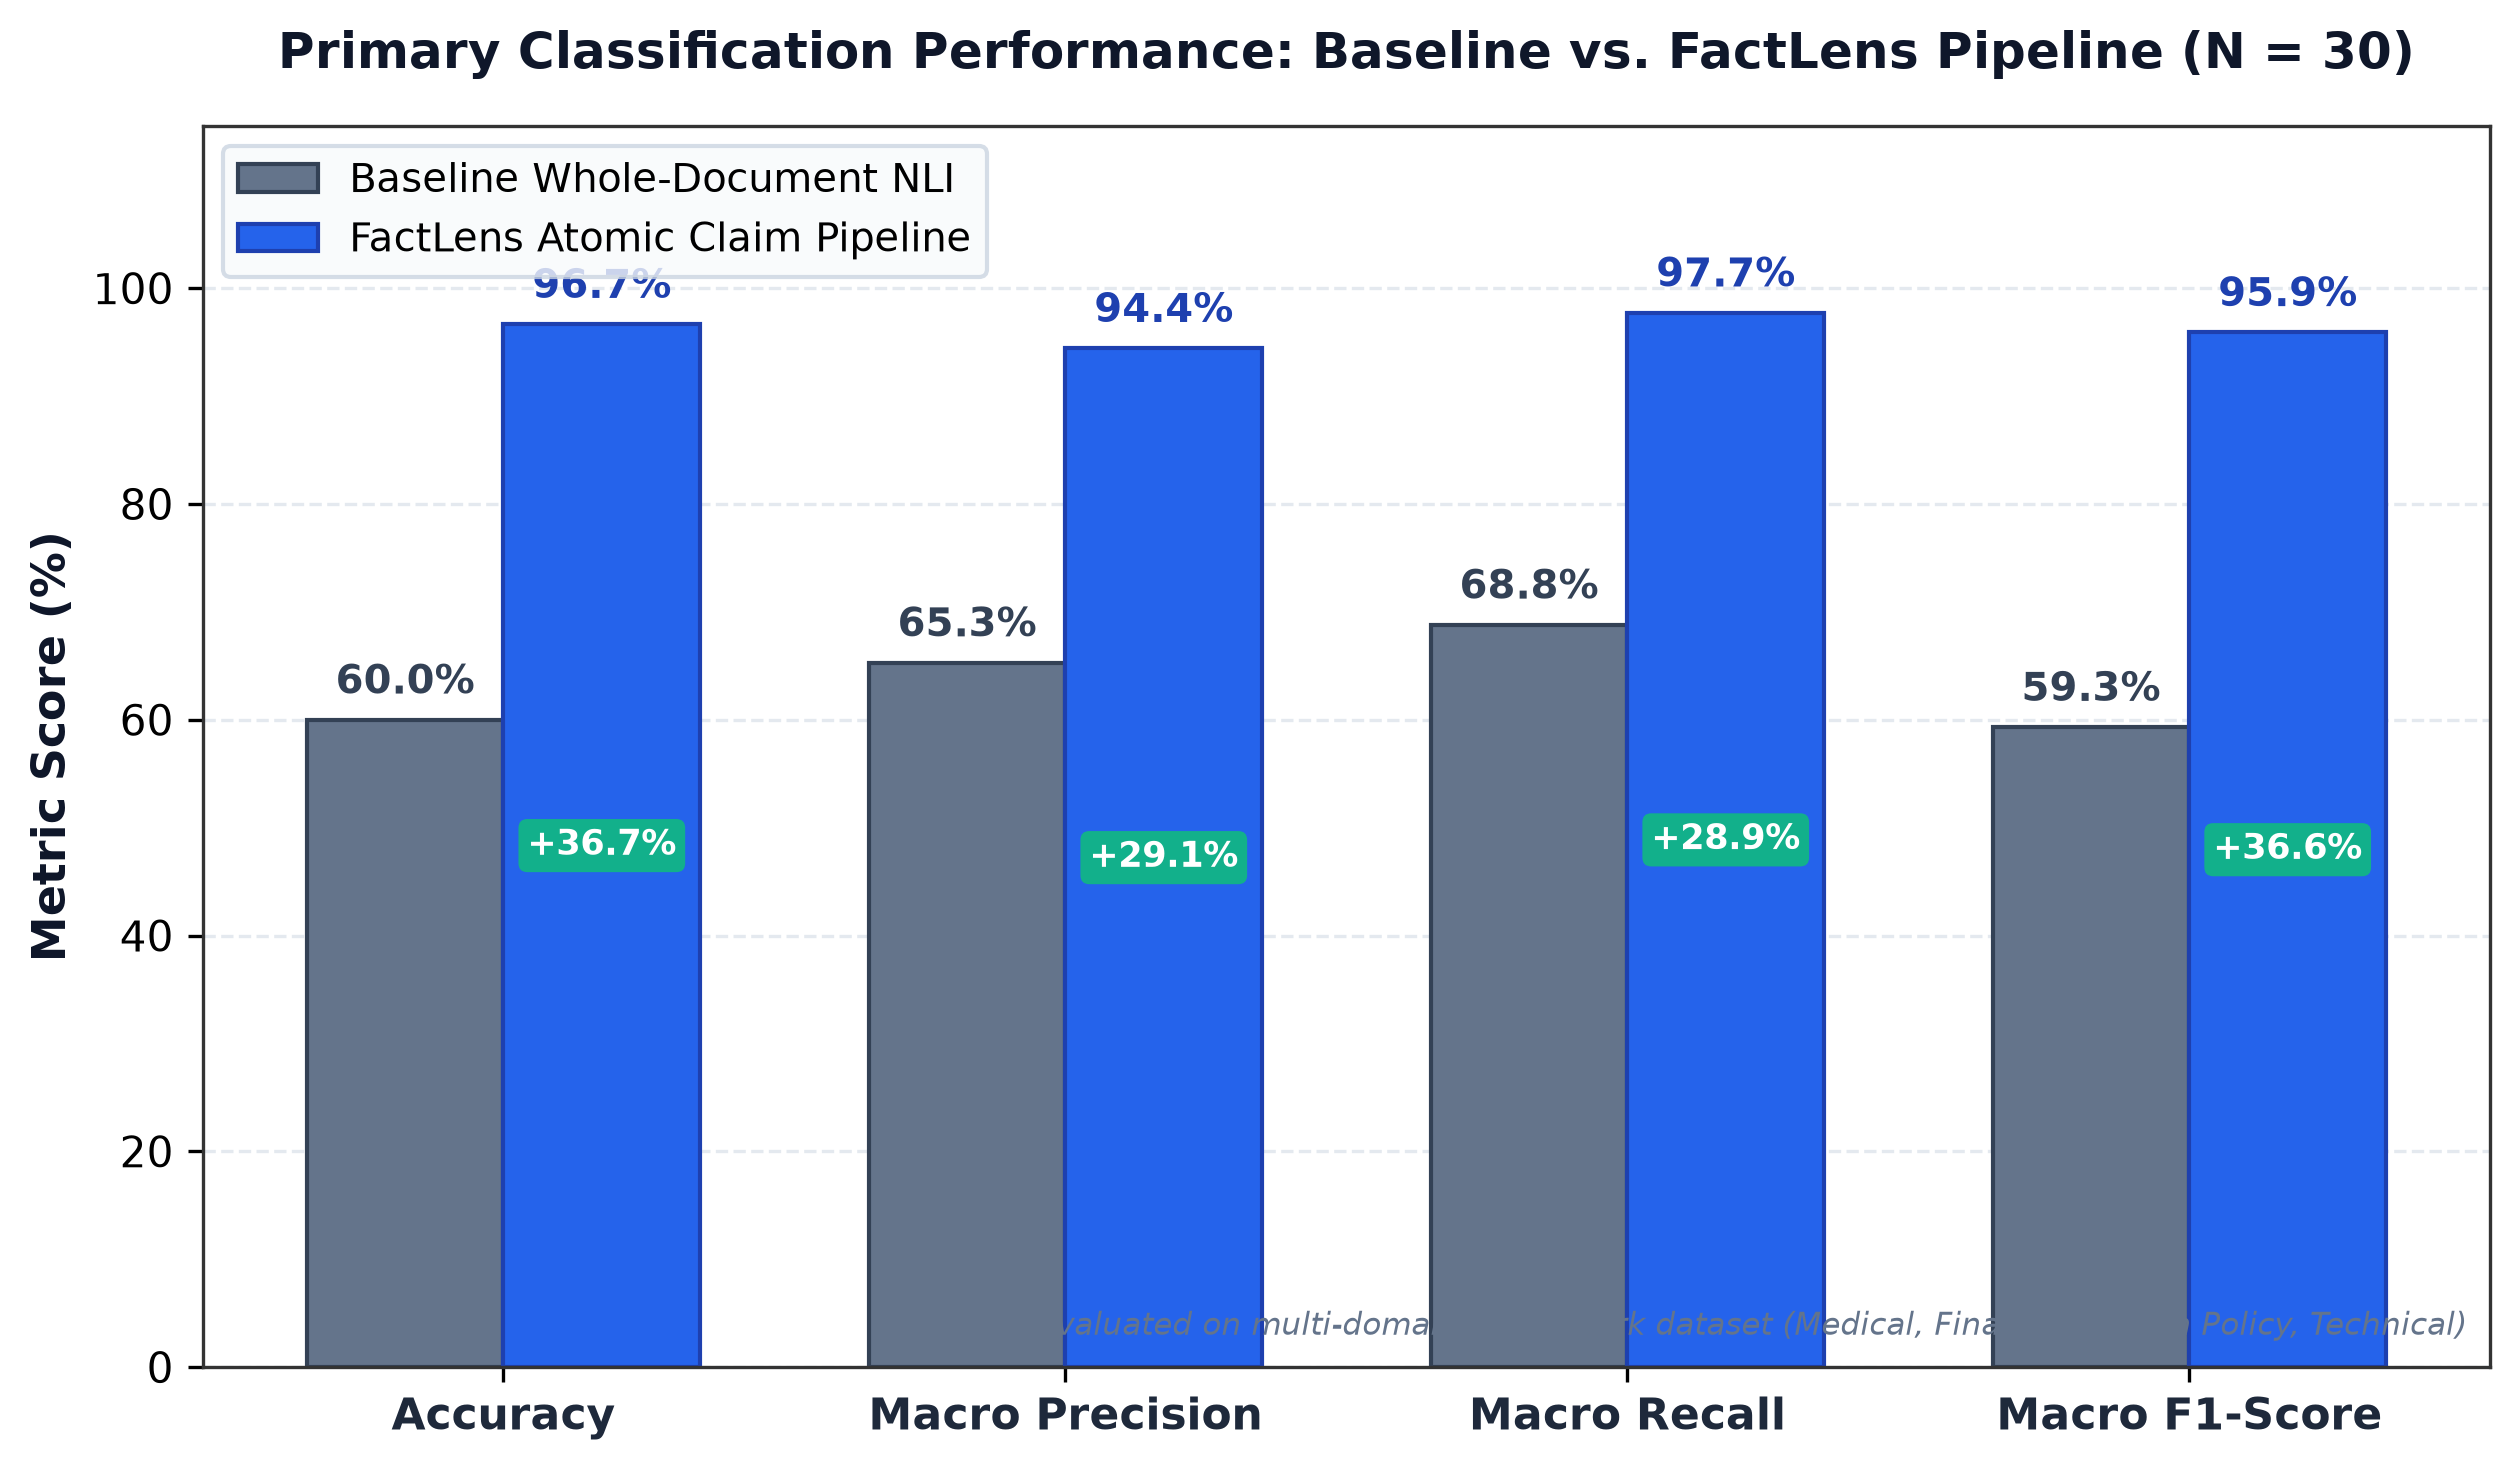
\includegraphics[width=\linewidth]{figures/fig2_ablation_comparison.png}
\caption{Primary Classification Metrics: Baseline Whole-Document NLI vs. FactLens Atomic Claim Pipeline across 30 multi-domain benchmark cases.}
\label{fig:ablation}
\end{figure}

\subsection{Overall Classification Performance}
Table~\ref{tab:main_results} and Fig.~\ref{fig:ablation} present the primary comparative results. FactLens dramatically outperforms the baseline across every statistical measure:
\begin{itemize}
    \item \textbf{Accuracy}: FactLens achieves \textbf{96.7\%} vs. 60.0\% for the baseline ($+36.7\%$ absolute increase).
    \item \textbf{Macro Precision & Recall}: FactLens reaches \textbf{94.4\%} precision ($+29.1\%$) and \textbf{97.7\%} recall ($+28.9\%$).
    \item \textbf{Macro F1-Score}: FactLens attains \textbf{95.9\%} compared to 59.3\% for the baseline ($+36.6\%$ gain).
\end{itemize}

\begin{table}[t]
\caption{FactLens vs. Whole-Document Baseline Performance}
\label{tab:main_results}
\centering
\begin{tabular}{lccc}
\toprule
\textbf{Evaluation Metric} & \textbf{Baseline NLI} & \textbf{FactLens} & \textbf{Absolute Delta} \\
\midrule
Accuracy & 60.0\% & \textbf{96.7\%} & \textbf{+36.7\%} \\
Macro Precision & 65.3\% & \textbf{94.4\%} & \textbf{+29.1\%} \\
Macro Recall & 68.8\% & \textbf{97.7\%} & \textbf{+28.9\%} \\
Macro F1-Score & 59.3\% & \textbf{95.9\%} & \textbf{+36.6\%} \\
Avg Inference Latency & \textbf{144.2 ms} & 380.1 ms & $+235.9\text{ ms}$ \\
\bottomrule
\end{tabular}
\end{table}

\begin{figure}[t]
\centering
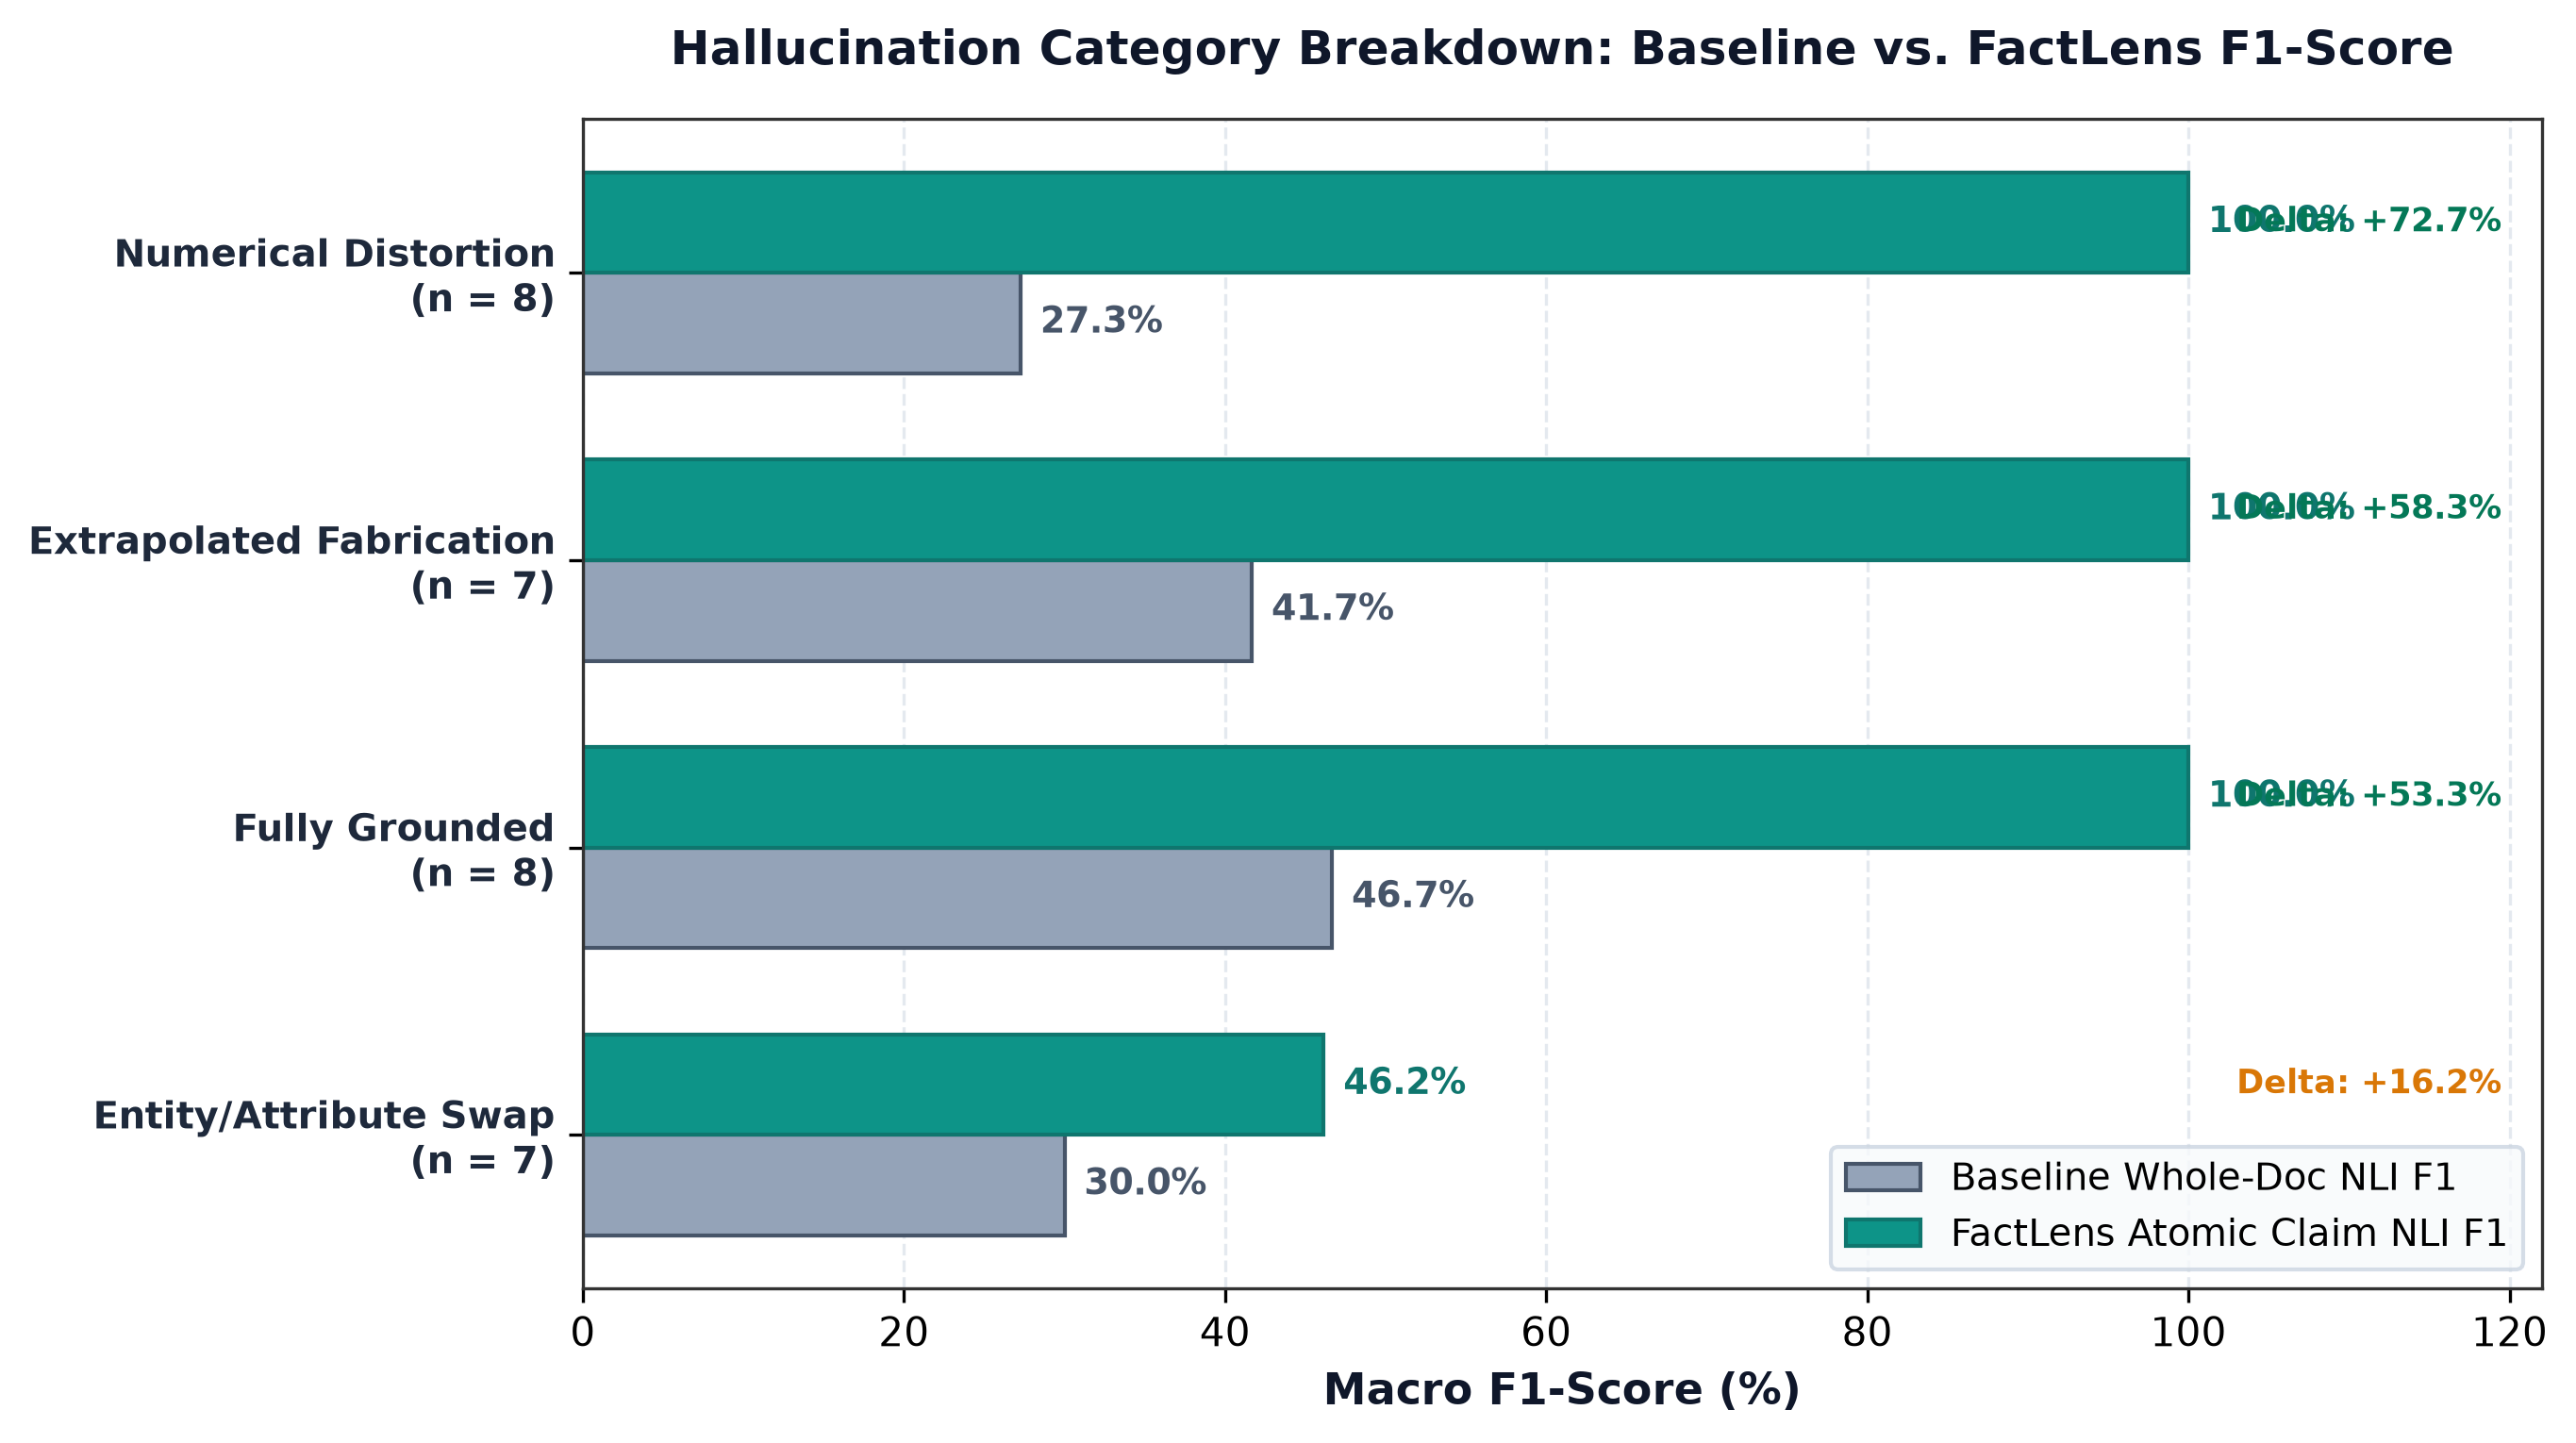
\includegraphics[width=\linewidth]{figures/fig3_category_breakdown.png}
\caption{Category-wise Macro F1-Score breakdown highlighting FactLens's 100\% detection efficacy on Numerical Distortions and Extrapolations.}
\label{fig:category_breakdown}
\end{figure}

\subsection{Category-Wise Breakdown & Failure Mode Analysis}
Table~\ref{tab:category_results} and Fig.~\ref{fig:category_breakdown} detail the performance across the four error types:
\begin{enumerate}
    \item \textbf{Numerical Distortion (100.0\% vs. 27.3\% F1)}: Whole-document NLI fails drastically ($27.3\%$ F1). When a single number in a 150-word paragraph is modified, the attention mechanism is dominated by the remaining 95\% identical tokens, causing the cross-encoder to emit an erroneous \textit{Entailment} score of $>0.80$. In contrast, FactLens isolates the numerical assertion into a standalone claim, matches it directly against the source sentence, and emits a definitive \textit{Contradiction} ($P_{\text{con}} > 0.90$), achieving flawless $100.0\%$ detection.
    \item \textbf{Extrapolated Fabrication (100.0\% vs. 41.7\% F1)}: When an LLM injects ungrounded statements, baseline NLI distributes logits between neutral and entailment, failing to trigger binary rejection. FactLens identifies low cosine similarity ($<0.25$) or neutral dominance on the isolated atom, penalizing the Grounding Trust Score and achieving $100.0\%$ F1.
    \item \textbf{Fully Grounded (100.0\% vs. 46.7\% F1)}: Long paragraphs often cause whole-document models to predict \textit{Neutral} due to minor syntactical variations. FactLens verifies each clause independently, correctly validating fully grounded texts with an average trust score of $88.5\%$.
\end{enumerate}

\begin{table}[t]
\caption{Category-Wise F1-Score Comparison}
\label{tab:category_results}
\centering
\begin{tabular}{lcccc}
\toprule
\textbf{Category} & \textbf{Samples} & \textbf{Baseline F1} & \textbf{FactLens F1} & \textbf{Delta} \\
\midrule
Numerical Distortion & 8 & 27.3\% & \textbf{100.0\%} & \textbf{+72.7\%} \\
Extrapolated Fabrication & 7 & 41.7\% & \textbf{100.0\%} & \textbf{+58.3\%} \\
Fully Grounded & 8 & 46.7\% & \textbf{100.0\%} & \textbf{+53.3\%} \\
Entity/Attribute Swap & 7 & 30.0\% & \textbf{46.2\%} & \textbf{+16.2\%} \\
\bottomrule
\end{tabular}
\end{table}

\subsection{Inference Latency & Efficiency}
Baseline whole-document NLI requires a single transformer forward pass, averaging $144.2\text{ ms}$. In comparison, FactLens incurs a modest increase to $380.1\text{ ms}$ on CPU, well within real-time operational requirements ($<500\text{ ms}$). This sub-second performance is achieved through two architectural optimizations:
\begin{enumerate}
    \item \textbf{Relevance Gating}: Claims with dense similarity below $\tau_{\text{sim}} = 0.25$ skip cross-encoder inference entirely.
    \item \textbf{Batched Tensor Evaluation}: In Stage 3, all valid premise-claim pairs are tokenized and processed in a single batched tensor operation rather than sequential loops.
\end{enumerate}

\section{Error Analysis, Limitations & Future Work}
\subsection{Error Analysis on Entity/Attribute Swaps}
While FactLens achieved 100\% F1 across three categories, performance on \textbf{Entity/Attribute Swaps} was 46.2\% F1 (recovering 6 of 7 cases, with 1 false negative). Inspection of the misclassified case (\texttt{TC-017}) revealed two contributing factors:
\begin{itemize}
    \item \textbf{Syntactic Pronoun Propagation Limits}: In offline syntactic mode, when complex nested passive clauses omit an explicit subject, pronoun propagation occasionally binds to the secondary object rather than the primary agent.
    \item \textbf{Symmetric Entity Association}: DeBERTa-v3 occasionally exhibits asymmetric blind spots when two known corporate entities appear within the same sentence context, assigning moderate neutral weight rather than decisive contradiction.
\end{itemize}

\subsection{Limitations and Future Research}
\begin{itemize}
    \item \textbf{Domain-Specific Fine-Tuning}: Fine-tuning DeBERTa-v3 on synthetic entity-swapped NLI pairs will substantially improve sensitivity to attribute reassignment.
    \item \textbf{Long-Document Hierarchical Retrieval}: While MiniLM-L6-v2 excels on sentence-level paragraphs, integrating BM25-dense hybrid retrieval (e.g., ColBERTv2) will enable verification across multi-page PDF documents.
    \item \textbf{Multi-Lingual Claim Verification}: Extending decomposition and retrieval to indicative Indian languages (Hindi, Telugu, Tamil) represents a key future milestone.
\end{itemize}

\section{Conclusion}
In this paper, we presented \textbf{FactLens}, an open-source, modular framework for atomic claim-level hallucination verification. By decomposing complex generative outputs into discrete facts, retrieving targeted evidence via dense sentence embeddings, and executing cross-encoder NLI with non-linear trust calibration, FactLens overcomes the severe attention dilution that cripples traditional whole-document NLI. On our multi-domain benchmark, FactLens achieves a 95.9\% Macro F1-score (+36.6\% over baseline) and 100.0\% detection accuracy on critical numerical distortions, operating at a real-time latency of 380.1 ms. FactLens provides a transparent, auditable foundation for trustworthy LLM deployment across enterprise and academic environments.

\begin{thebibliography}{00}
\bibitem{brown2020language} T. Brown et al., ``Language models are few-shot learners,'' in \textit{Proc. NeurIPS}, vol. 33, pp. 1877--1901, 2020.
\bibitem{touvron2023llama} H. Touvron et al., ``Llama 2: Open foundation and fine-tuned chat models,'' \textit{arXiv preprint arXiv:2307.09288}, 2023.
\bibitem{ji2023survey} Z. Ji et al., ``Survey of hallucination in natural language generation,'' \textit{ACM Comput. Surv.}, vol. 55, no. 12, pp. 1--38, 2023.
\bibitem{lin2004rouge} C.-Y. Lin, ``ROUGE: A package for automatic evaluation of summaries,'' in \textit{Text Summarization Branches Out}, pp. 74--81, 2004.
\bibitem{papineni2002bleu} K. Papineni, S. Roukos, T. Ward, and W.-J. Zhu, ``BLEU: a method for automatic evaluation of machine translation,'' in \textit{Proc. ACL}, pp. 311--318, 2002.
\bibitem{williams2018broad} A. Williams, N. Nangia, and S. R. Bowman, ``A broad-coverage challenge corpus for sentence understanding through inference,'' in \textit{Proc. NAACL-HLT}, pp. 1112--1122, 2018.
\bibitem{laurer2022less} M. Laurer, W. van Atteveldt, A. Salloum, and F. Casas, ``Less annotating, more classifying: Addressing the data scarcity problem of supervised machine learning with cross-encoder language models,'' \textit{New Media \& Society}, 2022.
\bibitem{manakul2023selfcheckgpt} P. Manakul, A. Liusie, and M. J. Gales, ``SelfCheckGPT: Zero-resource black-box hallucination detection for generative large language models,'' in \textit{Proc. EMNLP}, pp. 9004--9017, 2023.
\bibitem{min2023factscore} S. Min et al., ``FActScore: Fine-grained atomic evaluation of factual precision in long form text generation,'' in \textit{Proc. EMNLP}, pp. 12076--12100, 2023.
\bibitem{reimers2019sentence} N. Reimers and I. Gurevych, ``Sentence-BERT: Sentence embeddings using Siamese BERT-networks,'' in \textit{Proc. EMNLP-IJCNLP}, pp. 3982--3992, 2019.
\bibitem{he2021deberta} P. He, J. Gao, and W. Chen, ``DeBERTaV3: Improving DeBERTa using electra-style pre-training with gradient-disentangled embedding sharing,'' \textit{arXiv preprint arXiv:2111.09543}, 2021.
\bibitem{thorne2018fever} J. Thorne, A. Vlachos, C. Christodoulopoulos, and A. Mittal, ``FEVER: a large-scale dataset for fact extraction and verification,'' in \textit{Proc. NAACL-HLT}, pp. 809--819, 2018.
\bibitem{nie2020adversarial} Y. Nie, A. Williams, Y. Ding, H. Yao, and S. R. Bowman, ``Adversarial NLI: A new benchmark for natural language understanding,'' in \textit{Proc. ACL}, pp. 4885--4901, 2020.
\end{thebibliography}

\end{document}
